% !TEX root = 99_main.tex

To study the electricity generation and building energy consumption a 3D geometry of the room and solar facade is built using the Rhinoceros \cite{Rhino}, and its parametric modelling plugin Grasshopper \cite{grasshopper}. In our case the room is XX meters in length, YY meters wide, and X meters high. The solar facade consists of 400mm CIGS square panels that can rotate in two degrees of freedom. On the horizontal axis it can move from 90$^{\circ}$ (closed) to 0$^{\circ}$ (open) position in steps of 15$^{\circ}$, in the vertical axis it can move from 45$^{\circ}$ to -45$^{\circ}$ in steps of 15$^{\circ}$. This leaves us with \textcolor{red}{49} possible dynamic configurations of the facade system. 

The building energy simulation is conducted using Energy Plus \cite{energyplus} through the DIVA \cite{DIVA} interface. The geometric solar facade is interpreted in energyplus as an external shading system. A solar radiance simulation is run in parallel using ladybug [Citation required] to determine the incident insolation on the solar facade. Reflected and diffuse light are taken into account using the global radiation data, visible sky fraction for each panel, and the reflection of surrounding elements. The results enables us to calculate the electricity generation, while taking into account aspects of self shading. 

A simulation of each possible dynamic configuration of the facade is run for each hourly timestep of the year using the Geneva weather file. The results are then post processed in Python to extract the configurations that minimized building energy consumption while maximising PV electricity production. 

\begin{figure}
\begin{center}
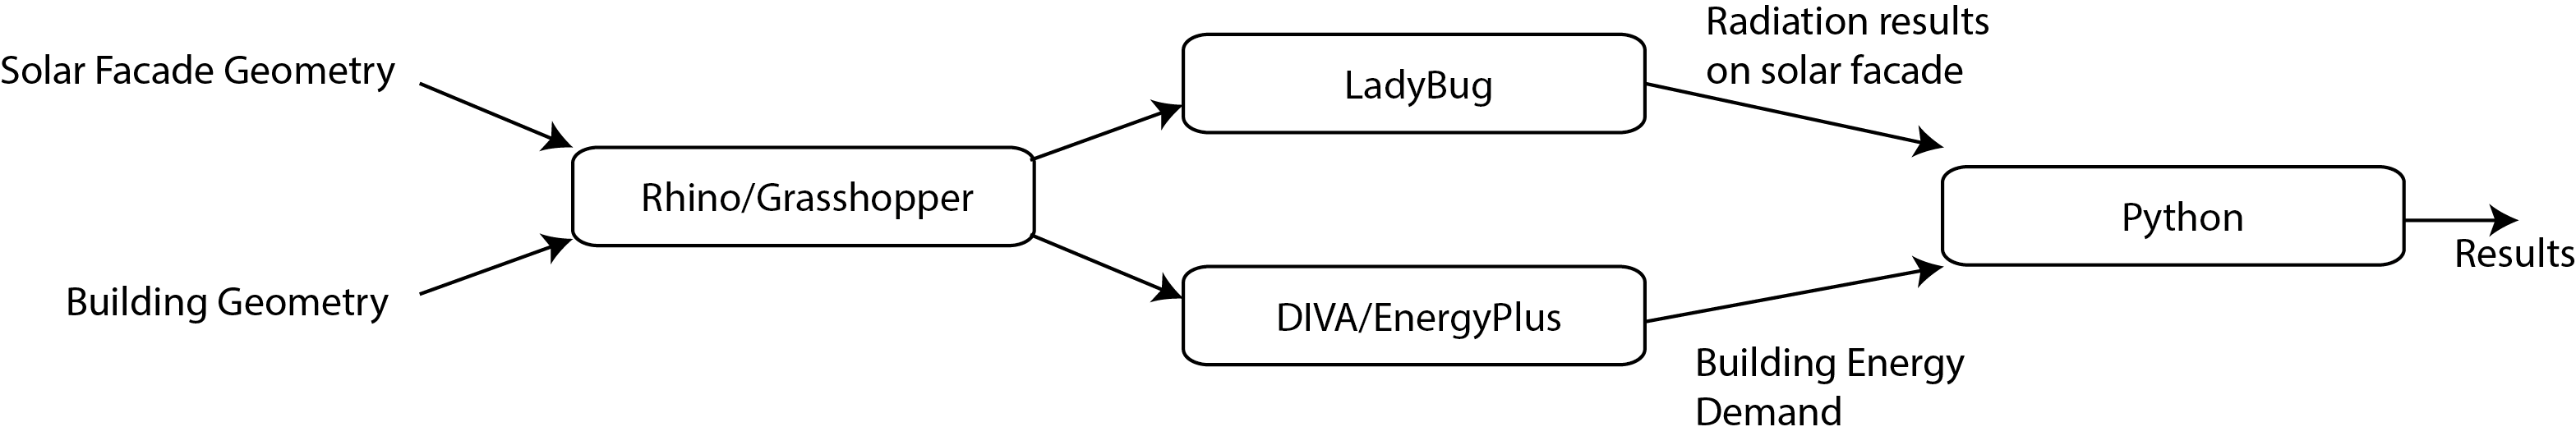
\includegraphics[width=15cm, trim= 0cm 0cm 0cm 0cm,clip]{workflow.png}
\caption{Workflow of the simulation (rough)}
\label{fig:workflow}
\end{center}
\end{figure}